\documentclass[submit]{harvardml}

% FDV: Make sure all front matter has correct years, dates, book sections, etc.
\course{CS181-S22}
\assignment{Assignment \#2}
\duedate{7:59pm EST, Feb 25th, 2022}

\usepackage[OT1]{fontenc}
\usepackage[colorlinks,citecolor=blue,urlcolor=blue]{hyperref}
\usepackage[pdftex]{graphicx}
\usepackage{subfig}
\usepackage{fullpage}
\usepackage{amsmath}
\usepackage{amssymb}
\usepackage{framed}
\usepackage{color}
\usepackage{soul}
\usepackage{todonotes}
\usepackage{listings}
\usepackage{common}
\usepackage{enumitem}
\usepackage{bm}
\newcommand{\B}{\text{B}}
\newcommand{\Beta}{\text{Beta}}

\usepackage[mmddyyyy,hhmmss]{datetime}

\definecolor{verbgray}{gray}{0.9}

\lstnewenvironment{csv}{%
  \lstset{backgroundcolor=\color{verbgray},
  frame=single,
  framerule=0pt,
  basicstyle=\ttfamily,
  columns=fullflexible}}{}

\begin{document}

\begin{center}
{\Large Homework 2: Classification and Bias-Variance Trade-offs}\\
\end{center}

\subsection*{Introduction}

This homework is about classification and bias-variance trade-offs. In
lecture we have primarily focused on binary classifiers trained to
discriminate between two classes. In multiclass classification, we
discriminate between three or more classes.  Most of the material for Problem 1 and Problem 3, and all of the material for Problem 2 will be covered by the end of the Tuesday 2/8 lecture. The rest of the material will be covered by the end of the Thursday 2/10 lecture.  We encourage you to read
CS181 Textbook's Chapter 3 for more information on linear
classification, gradient descent, classification in the discriminative
setting (covers multiclass logistic regression and softmax), and
classification in the generative setting. Read Chapter 2.8 for more
information on the trade-offs between bias and variance.

As a general note, for classification problems we imagine that we have
the input matrix $\boldX \in \reals^{N \times D}$ (or perhaps they
have been mapped to some basis $\bm{\Phi}$, without loss of
generality) with outputs now ``one-hot encoded."  This means that if
there are~$K$ output classes, rather than representing the output
label $y$ as an integer~${1,2,\ldots,K}$, we represent $\boldy$ as a
``one-hot" vector of length~$K$. A ``one-hot" vector is defined as
having every component equal to 0 except for a single component which
has value equal to 1.  For example, if there are $K = 7$ classes and a
particular data point belongs to class 3, then the target vector for
this data point would be~$\boldy = [0,0,1,0,0,0,0]$.  We will define
$C_1$ to be the one-hot vector for the 1st class, $C_2$ for the 2nd
class, etc.  Thus, in the previous example $\boldy = C_3$. If there
are $K$ total classes, then the set of possible labels is $\{C_1
\ldots C_K \} = \{C_k\}_{k=1}^K$.  Throughout the assignment we will
assume that each label $\boldy \in \{C_k\}_{k=1}^K$ unless otherwise
specified. The most common exception is the case of binary classification
($K = 2$), in which case labels are the typical integers $y \in \{0, 1\}$.\\

In problems 1 and 3, you may use \texttt{numpy} or \texttt{scipy}, but
not \texttt{scipy.optimize} or \texttt{sklearn}. Example code given is
in Python 3.\\

Please type your solutions after the corresponding problems using this
\LaTeX\ template, and start each problem on a new page.\\

Please submit the \textbf{writeup PDF to the Gradescope assignment `HW2'}. Remember to assign pages for each question.  \textbf{You must include your plots in your writeup PDF. } The supplemental files will only be checked in special cases, e.g. honor code issues, etc. \\

Please submit your \textbf{\LaTeX\ file and code files to the Gradescope assignment `HW2 - Supplemental'}. 

%%%%%%%%%%%%%%%%%%%%%%%%%%%%%%%%%%%%%%%%%%%%%
% Problem 1
%%%%%%%%%%%%%%%%%%%%%%%%%%%%%%%%%%%%%%%%%%%%%

\begin{problem}[Exploring Bias and Variance, 10 pts]
  In this problem, we will explore the bias and variance of a
  few different model classes when it comes to logistic regression.

  Consider the true data generating process $y \sim \text{Bern}(f(x)), f(x) = 0.4 \times \sin(1.2x) + 0.5$, where $x \in [-3, 3]$, and $y \in \{0,1\}$.
  Recall that for a given $x$, bias and variance are defined in terms of expectations \textit{over randomly drawn datasets} $D$
  from this underlying data distribution:
  \begin{align*}
  \text{Bias}[\hat{f}(x)] &= \mathbb{E}_D[\hat{f}(x)] - f(x)\\
  \text{Variance}[\hat{f}(x)] &= \mathbb{E}_D[(\hat{f}(x) - \mathbb{E}_D[\hat{f}(x)])^2]
  \end{align*}
  Here, $\hat{f}(x)$ is our estimator (learned through logistic
  regression on a given dataset $D$).  We will directly explore the
  bias-variance trade-off by drawing multiple such datasets and
  fitting different logistic regression models to each.  Remember that
  we, the modelers, do not usually see the true data distribution.
  Knowledge of the true $f(x)$ is only exposed in this problem to (1)
  make possible the simulation of drawing multiple datasets, and (2)
  to serve as a pedagogical tool in allowing verification of the true
  bias.

\begin{enumerate}

\item Consider the three bases $\phi_1(x) = [1, x]$, $\phi_2(x) = [1,
  x, x^2]$, $\phi_3(x) = [1, x, x^2, x^3, x^4, x^5]$.  For each
  of these bases, generate 10 datasets of size $N = 30$ using the
  starter code provided, and fit a logistic regression model using
  sigmoid($w^T \phi(x)$) to each dataset by using gradient descent to
  minimize the negative log likelihood.  This means you will be
  running gradient descent 10 times for each basis, once for each
  dataset.  Note that the classes are represented with 0's and 1's.
  
  Use random starting values of $w$, $\eta=0.001$, take 10,000 update
  steps for each gradient descent run, and make sure to average the
  gradient over the data points (for each step). These parameters,
  while not perfect, will ensure your code runs in a reasonable amount
  of time. The emphasis of this problem is on capturing the
  bias-variance trade-off, so don't worry about attaining perfect
  precision in the gradient descent as long as this trade-off is
  captured in the final models.

   Note: Overflow RuntimeWarnings due to \verb|np.exp| should be safe to ignore, if any. Also, to reduce stress from randomness in students' solutions (due to randomized weight initialization differences), in line $109$ of the \verb|T2_P1.py| starter code, we call \verb|np.random.seed(1738)| to set a deterministic random seed. Please do not change this! In addition, please do not change the randomized weight initialization code in lines $42-46$.

\item Create three plots, one for each basis. Starter code is available which you may modify.
By default, each plot displays three types of functions:
(1) the true data-generating distribution $f(x)$ (the probability that $y=1$ for different $x$).
(2) all 10 of the prediction functions learned from each randomly drawn dataset, and
(3) the mean of the 10 prediction functions.
Moreover, each plot also displays 1 of the randomly generated datasets and highlights the corresponding prediction function learned by this dataset.

\item How are bias and variance reflected in the 3 types of curves on
  the graphs?  How do the fits of the individual and mean prediction
  functions change?  Keeping in mind that none of the model classes
  match the true generating process exactly, discuss the extent to
  which each of the bases approximates the true process.

  Note: In this problem, we are not interested in whether the model is
  more biased for certain inputs $x$ compared to other inputs $x'$.
  We are interested in the overall bias and variance of $\hat{f}(x)$
  across the different basis choices. In other words, we want to investigate how the bias between $\hat{f}(x)$ and the ground truth as well as the variance of $\hat{f}(x)$ will be different over different basis choices. 

\item If we were to increase the size of each dataset drawn from $N = 30$ to a larger number, how would the variance change? The bias?   Why might this be the case?

\end{enumerate}

\end{problem}

\newpage

\subsection*{Solution}

\begin{enumerate}

\item 

This part of the problem is implemented in T2\_P1.py

\item

Below are the three plots, each separated on a different page.

\newpage
\begin{figure}[h]
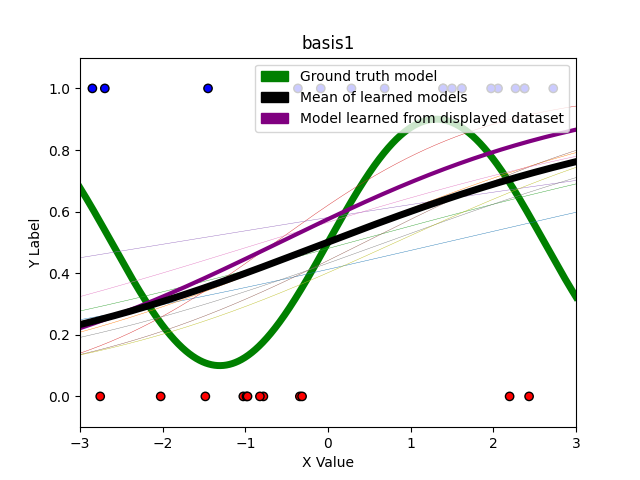
\includegraphics[scale=0.8]{basis1}
\centering
\end{figure}
\newpage

\begin{figure}[h]
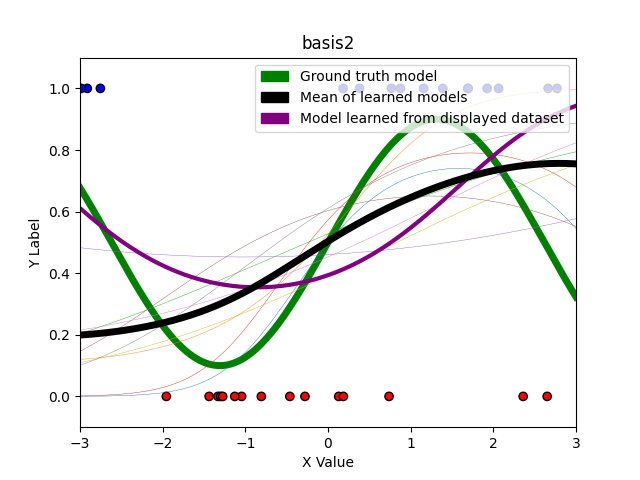
\includegraphics[scale=0.8]{basis2}
\centering
\end{figure}
\newpage

\begin{figure}[h]
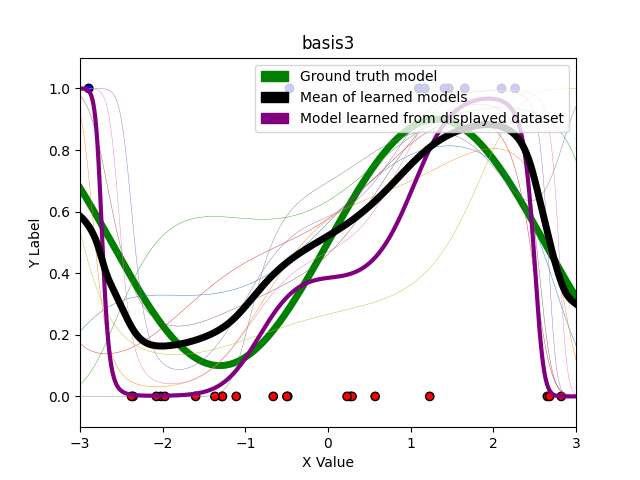
\includegraphics[scale=0.8]{basis3}
\centering
\end{figure}
\newpage

\item

\textbf{How are bias and variance reflected in the 3 types of curves on the graphs?}

Bias and variance are reflected in the 3 types of curves on the graphs by

1. How much models of a given type vary when new datasets are used (e.g., how
different the thin lines on the graph are from each other). This visual component
corresponds to the variance of the models. 

2. How a single given model fits the dataset (e.g., how well the purple line, 
which was fit using the displayed dataset, fit to the displayed dataset))). This
visual component corresponds to the bias of models.

\textbf{How do the fits of the individual and mean prediction functions change?}

For the simpler models, such as those that use basis1, the individual predictions functions don't
vary all that much. As the complexity increases when we move on to basis2 and basis3, 
individual prediction functions begin to vary a lot more from each other. This 
is due to the ability of the more complex models to fit their curves to 
correctly classify a given dataset.

As for the mean prediction functions, they become significantly more accurate as we move 
on to more complex bases. The mean prediction function for models that use basis3
very closely resembles the ground truth model. It is clear in this case, however
that it is only the mean prediction function that is accurate and not the individual models that 
are accurate, as the model learned from the displayed dataset (in purple in the plot
for basis3) is very clearly fitting its dataset much more closely than it is resembling 
the ground truth model. 

\textbf{Keeping in mind that none of the bases approximates
the true generating process exactly, discuss the extent to which each of the bases
approximates the true process.}

basis1 is unable to approximate the true process which much accuracy at all as it 
is simply unable to model the form of the true process with only 
non-quadratic terms of the $x$-values.

basis2 is not too accurate for the same reason, however, it does have slightly less bias 
and more variance. 

basis3 is able to approximate the true process very well as it uses a more complete
polynomial of $\textbf{x}$ as its basis. It does tend, however, to fit more closely
to the data points themselves than to the true process, which is the downside of this basis.

\item 
Increasing the dataset size would \textbf{decrease} the variance, given that models
would be required to use their weights to fit across more points. This is the 
opposite of what would happen if the dataset size were to be decreased, which 
would enable the models (especially those fit using basis3) to over-fit their 
weights for the data points available. The loss for this scenario may even become zero,
as basis3 could exactly fit a low enough given amount of data points.

As for the bias, increasing the dataset size would \textbf{decrease} the bias as 
each model would be given more information from which to tune their weights. More
technically speaking, gradient descent would be able to take advantage of much
more accurate gradients when optimizing weights.

\end{enumerate}

%%%%%%%%%%%%%%%%%%%%%%%%%%%%%%%%%%%%%%%%%%%%%
% Problem 2
%%%%%%%%%%%%%%%%%%%%%%%%%%%%%%%%%%%%%%%%%%%%%

\begin{problem}[Maximum likelihood in classification, 15pts]

  Consider now a generative $K$-class model.  We adopt class prior
  $p(\boldy = C_k; \bpi) = \pi_k$ for all $k \in \{1, \ldots, K\}$
(where $\pi_k$ is a parameter of the prior).
Let  $p(\boldx|\boldy=C_k)$ denote
the class-conditional density of features $\boldx$ (in this
case for class $C_k$). Consider the data set $D = \{(\boldx_i,
\boldy_i)\}_{i=1}^n$ where as above $\boldy_i \in \{C_k\}_{k=1}^K$ is
encoded as a one-hot target vector and the data are independent.

\begin{enumerate}
  \item Write out the log-likelihood of the data set, $\ln p(D ; \bpi)$.

  \item Since the prior forms a distribution, it has the constraint that
    $\sum_k\pi_k - 1 = 0$.  Using the hint on
Lagrange multipliers below, give the
    expression for the maximum-likelihood estimator for the prior
    class-membership probabilities, i.e.
    $\hat \pi_k.$
    Make sure to write out the intermediary equation you need
    to solve to obtain this estimator. Briefly state why your final answer is intuitive.
\end{enumerate}

    For the remaining questions, let the
    class-conditional probabilities be Gaussian distributions with
the same covariance matrix
    $$p(\boldx | \boldy = C_k) = \mathcal{N}(\boldx |  \bmu_k, \bSigma), \text{\ for\ }k \in \{1,\ldots, K\}$$
    and different means $\bmu_k$ for each class.

    \begin{enumerate}
  \item[3.] Derive the gradient of the log-likelihood with respect to vector $\bmu_k$.
    Write the expression in matrix form as a function of the variables defined
    throughout this exercise. Simplify as much as possible for full credit.
  \item[4.] Derive the maximum-likelihood estimator $\hat{\mu}_k$ for vector $\bmu_k$. Briefly state why your final answer is intuitive.
  \item[5.] Derive the gradient for the log-likelihood with respect to the
    covariance matrix $\bSigma$ (i.e., looking
to find an MLE for the covariance).
Since you are differentiating with respect to a
    \emph{matrix}, the resulting expression should be a matrix!
%
  \item[6.] Derive the maximum likelihood estimator $\hat{\Sigma}$ of the covariance matrix.
\end{enumerate}

\paragraph{Hint: Lagrange Multipliers.} Lagrange Multipliers are a method for
optimizing a function $f$ with respect to an
equality constraint, i.e.
\[\min_{\boldx} f(\boldx)\ \text{s.t.}\ g(\boldx) = 0.\]

This can be turned into an unconstrained problem by introducing a
Lagrange multiplier $\lambda$ and constructing the Lagrangian function,
\[L(\boldx, \lambda) =  f(\boldx) + \lambda g(\boldx).\]

It can be shown that it is a necessary condition that the optimum
is a critical point of this new function. We can find this point by solving two equations:

\[\frac{\partial L(\boldx, \lambda)}{\partial  \boldx} = 0  \ \ \text{and}\  \  \frac{\partial L(\boldx, \lambda)}{\partial \lambda} = 0 \]


\paragraph{Cookbook formulas.} Here are some formulas you might want to consider
using to compute difficult gradients. You can use them  in the homework
without proof. If you are looking to hone your matrix calculus skills, try to
find different ways to prove these formulas yourself (will not be part of the
evaluation of this homework). In general, you can use any formula from the matrix cookbook,
as long as you cite it. We opt for the following common notation:
$\boldX^{-\top} := (\boldX^{\top})^{-1}$
\begin{align*}
  & \frac{\partial \bolda^\top \boldX^{-1} \boldb}{\partial \boldX} = - \boldX^{-\top} \bolda \boldb^\top \boldX^{-\top} \\
  & \frac{\partial \ln | \det (\boldX) |}{\partial \boldX} = \boldX^{-\top}
 \end{align*}
 \end{problem}


\subsection*{Solution}

\begin{enumerate}
\item 

For each data point $(\boldx_i, \boldy_i)\in \{(\boldx_i, \boldy_i)\}_{i=1}^N$
we have
$$p(\boldx_i, C_k) = p(\boldy_i = C_k | \pi)p(\boldx_i | \boldy_i = C_k)$$
$$= \pi_k p(\boldx_i | \boldy_i = C_k)$$
making the likelihood of the data set
$$p(D; \pi) = p( \{(\boldx_i, \boldy_i)\}_{i=1}^N; \pi)$$
$$ = \prod_{i=1}^N \prod_{j=1}^K (\pi p(\boldx_i | \boldy_i = C_k))^{y_{ij}}$$

where $y_{ij} = 1$ if $y_i = C_j$ and is zero otherwise.

\item 




\end{enumerate}

%%%%%%%%%%%%%%%%%%%%%%%%%%%%%%%%%%%%%%%%%%%%%
% Problem 3
%%%%%%%%%%%%%%%%%%%%%%%%%%%%%%%%%%%%%%%%%%%%%

\begin{problem}[Classifying Stars, 15pts]

You're tasked with classifying three different kinds of stars using their magnitudes and temperatures. See star.png for a plot of
the data, adapted from
\url{http://astrosci.scimuze.com/stellar_data.htm} and available as
\verb|data/hr.csv|, which you will find in the Github repository. \\

The CSV file has three columns: type, magnitude, and temperature. The
first few lines look like this:
\begin{csv}
Type,Magnitude,Temperature
Dwarf,-5.8,-0.35
Dwarf,-4.1,-0.31
...
\end{csv}

In this problem, you will code up 4 different classifiers for this task:
\begin{enumerate}[label=\alph*)]

\item \textbf{A three-class generalization of logistic regression},
  also known as softmax regression, in which you implement gradient
  descent on the negative log-likelihood. In Question 2 you will
  explore the effect of using different values for the learning rate
  $\eta$ (\texttt{self.eta}) and regularization strength $\lambda$
  (\texttt{self.lam}).  Make sure to include a bias term and to use L2
  regularization. See CS181 Textbook's Chapter 3.6 for details on  multi-class logistic regression and softmax. For your implementation, use the loss and gradient expressions provided there.

\item \textbf{A generative classifier with Gaussian class-conditional
  densities with a \textit{shared covariance} matrix} across all classes. 
  Feel free to re-use your Problem 2 results.
\item \textbf{Another generative classifier with Gaussian class-conditional densities , but now 
with a \textit{separate covariance} matrix} learned for each class. (Note: 
The staff implementation can switch between the two Gaussian generative classifiers with just a
few lines of code.)

\item \textbf{A kNN classifier} in which you classify based on the $k=1,3,5$ nearest neighbors and the following distance function: $$dist(star_1, star_2) = ((mag_1 - mag_2)/3)^2 + (temp_1 - temp_2)^2$$
where nearest neighbors are those with the smallest distances from a given point.

  Note 1: When there are more than two labels, no label may have the
  majority of neighbors.  Use the label that has the most votes among
  the neighbors as the choice of label. 

  Note 2: The grid of points for which you are making predictions
  should be interpreted as our test space.  Thus, it is not necessary
  to make a test point that happens to be on top of a training point
  ignore itself when selecting neighbors.

\end{enumerate}

After implementing the above classifiers, complete the following exercises:

\begin{enumerate}
    \item Plot the decision boundaries generated by each classifier for the dataset. Include them in your PDF. 
    Identify the similarities and differences among the classifiers. What explains the differences?

    \item For logistic regression only, make a plot with ``Number of
      Iterations" on the x-axis and ``Negative Log-Likelihood Loss" on
      the y-axis for several configurations of the hyperparameters
      $\eta$ and $\lambda$.  Specifically, try the values $0.05$,
      $0.01$, and $0.001$ for each hyperparameter.  Limit the number
      of gradient descent iterations to 200,000.  What are your final
      choices of learning rate ($\eta$) and regularization strength
      ($\lambda$), and why are they reasonable? How does altering
      these hyperparameters affect the ability to converge, the rate
      of convergence, and the final loss (a qualitative description is
      sufficient)? You only need to submit one plot for your final
      choices of hyperparameters.

      Note: The \emph{likelihood} of the model is the probability of
      data given the model---it should not include the regularization
      term.  The \emph{objective} is the combination of the likelihood
      and the regularizer.
      
    \item For both Gaussian generative models, report the negative log-likelihood loss. Which model has a lower loss, and why?
      For the separate covariance model, be sure to use
      the covariance matrix that matches the true class of each data
      point.
    
    \item Consider a star with Magnitude 6 and Temperature 2.
      To what class does each classifier assign this star? Do the
      classifiers give any indication as to whether or not you should
  trust them?
\end{enumerate}
\end{problem}

\newpage

\begin{framed}
\noindent\textbf{Problem 3} (cont.)\\


\textbf{Implementation notes:} Run the controller file, \texttt{T2\_P3.py},
to test your code. Write the actual implementations in the \texttt{GaussianGenerativeModel},
\texttt{LogisticRegression}, and \texttt{KNNModel} classes, which are defined in the three
\texttt{T2\_P3\_ModelName.py} files. These classes follow the same interface pattern
as sklearn. Their code
currently outputs nonsense predictions just to show the
high-level interface, so you should replace their \texttt{predict()} implementations.
You'll also need to modify the hyperparameter
values in \texttt{T2\_P3.py} for logistic regression.
\end{framed}


\subsection*{Solution}

\newpage
%%%%%%%%%%%%%%%%%%%%%%%%%%%%%%%%%%%%%%%%%%%%%
% Name and Calibration
%%%%%%%%%%%%%%%%%%%%%%%%%%%%%%%%%%%%%%%%%%%%%
\subsection*{Name}

\subsection*{Collaborators and Resources}
Whom did you work with, and did you use any resources beyond cs181-textbook and your notes?

\subsection*{Calibration}
Approximately how long did this homework take you to complete (in hours)?



\end{document}
